\documentclass{article}
\usepackage{bm}
\usepackage{amsmath}
\usepackage{graphicx}
\usepackage{mdwlist}
\usepackage[colorlinks=true]{hyperref}
\usepackage{geometry}
\usepackage{kotex}
\geometry{margin=1in}
\geometry{headheight=2in}
\geometry{top=2in}
\usepackage{palatino}
%\renewcommand{\rmdefault}{palatino}
\usepackage{fancyhdr}

\newcommand{\red}[1]{{\color{red} #1}}
\newcommand{\blue}[1]{{\color{blue} #1}}
\newcommand{\orange}[1]{{\color{orange} #1}}
\newcommand{\purple}[1]{{\color{purple} #1}}

%\pagestyle{fancy}
\rhead{}
\lhead{}
\chead{%
  {\vbox{%
      \vspace{2mm}
      \large
      Hardware System Design 4190.309A\hfill
\\
      Seoul National University
      \\[4mm]
      \textbf{Practice \#11. DMA (Direct Memory Access)}\\
      \textbf{Jiwon Lee, Sangjun Son}
    }
  }
}

%%%%%%%%%%%%%%%%%%%%%%%
\usepackage{xcolor}
\usepackage{listings}
\definecolor{vgreen}{RGB}{104,180,104}
\definecolor{vblue}{RGB}{49,49,255}
\definecolor{vorange}{RGB}{255,143,102}

\lstdefinestyle{c-style}
{
    language=C,
    basicstyle=\scriptsize\ttfamily,
    keywordstyle=\color{vblue},
    identifierstyle=\color{black},
    commentstyle=\color{vgreen},
    numbers=left,
    numberstyle=\tiny\color{black},
    numbersep=10pt,
    tabsize=8,
    moredelim=*[s][\colorIndex]{[}{]},
    literate=*{:}{:}1
}
\lstdefinestyle{python-style}
{
    language=Python,
    basicstyle=\scriptsize\ttfamily,
    keywordstyle=\color{vblue},
    identifierstyle=\color{black},
    commentstyle=\color{vgreen},
    numbers=left,
    numberstyle=\tiny\color{black},
    numbersep=10pt,
    tabsize=8,
    moredelim=*[s][\colorIndex]{[}{]},
    literate=*{:}{:}1
}

\makeatletter
\newcommand*\@lbracket{[}
\newcommand*\@rbracket{]}
\newcommand*\@colon{:}
\newcommand*\colorIndex{%
    \edef\@temp{\the\lst@token}%
    \ifx\@temp\@lbracket \color{black}%
    \else\ifx\@temp\@rbracket \color{black}%
    \else\ifx\@temp\@colon \color{black}%
    \else \color{vorange}%
    \fi\fi\fi
}
\makeatother

\usepackage{trace}
%%%%%%%%%%%%%%%%%%%%%%%

\usepackage{paralist}

\usepackage{todonotes}
\setlength{\marginparwidth}{2.15cm}

\usepackage{tikz}
\usetikzlibrary{positioning,shapes,backgrounds}

\begin{document}

\pagestyle{fancy}

\section*{Goal}
\begin{itemize*}
\item Compare data transfer using CDMA vs transferring data through CPU.
\item Compare performance between CDMA, conventional data transferring through CPU using \linebreak \texttt{gettimeofday()}.
\end{itemize*}
\begin{figure}[ht]
	\centering
	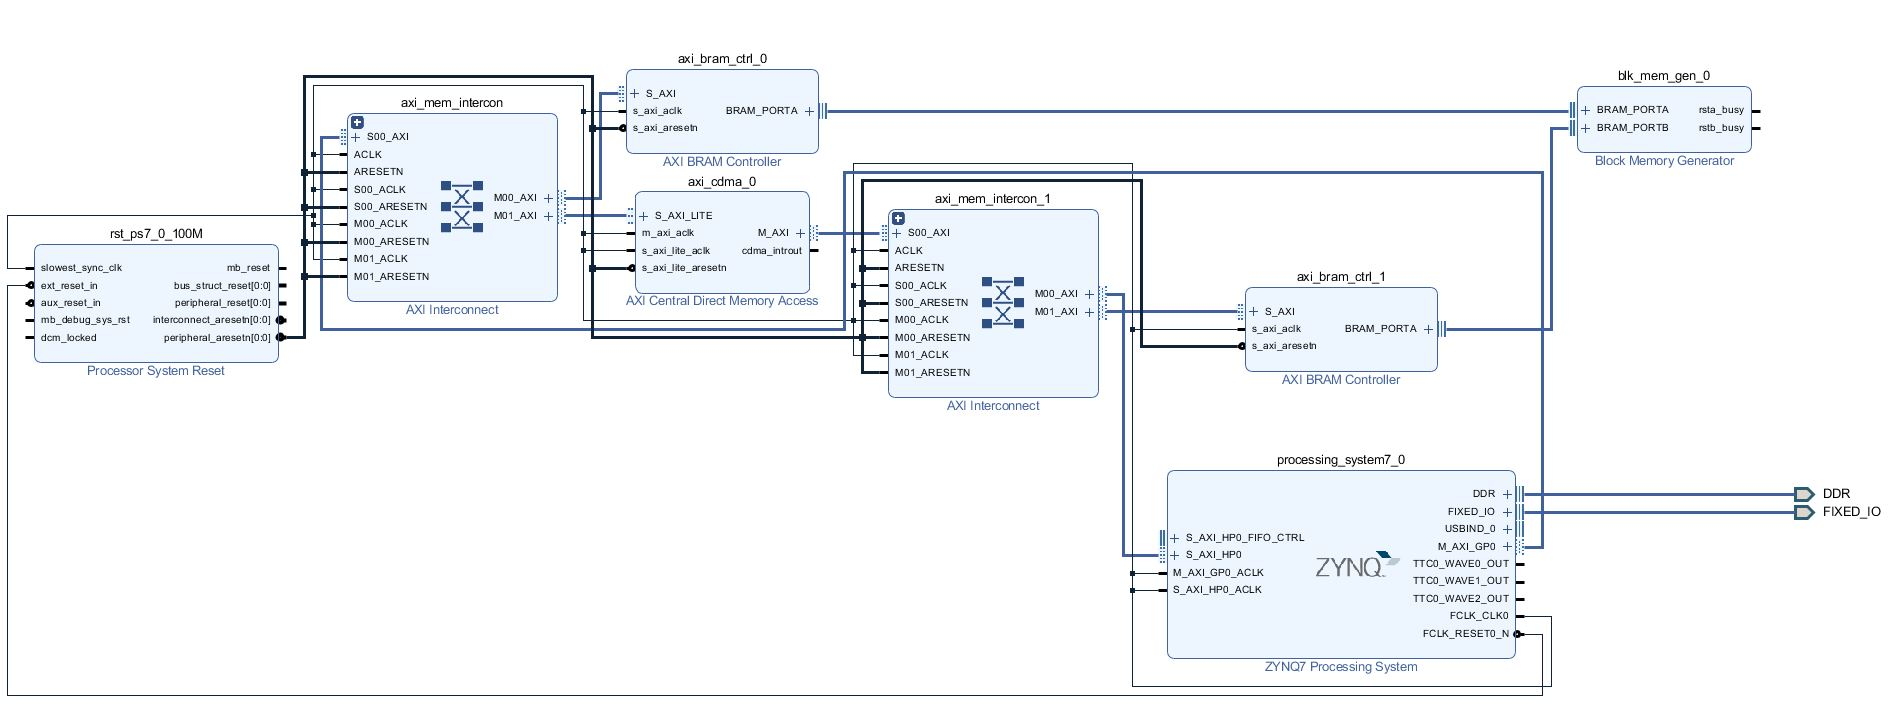
\includegraphics[width=1\textwidth]{fig/overview.jpg}
\caption{Memcopy and DMA Process with BRAM~\cite{lab11}.}
\label{fig1}
\end{figure}

\section{Implementation}
이번 랩에서는 Xilinx AXI CDMA(Central Direct Memory Accesss)를 이용하여 DMA를 수행해보고, 기존의 CPU를 통해 데이터를 쓰는 과정과 성능 면에서의 차이를 확인해본다. CDMA는 DRAM에서 BRAM(SRAM)으로 데이터를 쓰고, memcopy는 DRAM에서 DRAM으로 데이터를 쓴다. 하지만, CDMA는 CPU를 거치지 않기 때문에, memcopy보다 수행시간 측면에서 더 효율적이라는 것을 예상해 볼 수 있다. 또한, memcoppy와 memory load의 수행시간을 측정하여, 총 3가지 wrdata과정을 비교한다.\\\\
결론적으로, 이번 실습에서 비교해야 하는 Operation은 다음의 세 가지이다.
\begin{itemize}
  \setlength\itemsep{-0.5em}
    \item CDMA
    \item \texttt{memcpy()} in C
    \item Memory load
\end{itemize}

\begin{figure}[ht]
	\centering
	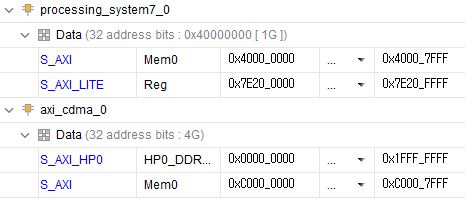
\includegraphics[width=1\textwidth]{fig/address.jpg}
\caption{Address of block elements}
\label{fig2}
\end{figure}
\newpage

아래는 보드에 매핑된 block element들의 주소와 이번 실습에서 performance 비교를 위한 C코드이다.
\subsection*{\texttt{CDMA}}
\begin{lstlisting}[style={c-style}]
struct timeval st[4];

// DMA : DRAM -> BRAM
unsigned int *fpga_dma = mmap(NULL, 16*sizeof(unsigned int), PROT_READ|PROT_WRITE, MAP_SHARED, foo, 0x7E200000);
gettimeofday (&st[2], NULL);
*(fpga_dma+6) = 0x10000000; // SA
*(fpga_dma+8) = 0xC0000000; // DA
*(fpga_dma+10) = SIZE * (SIZE + 1) * sizeof(float); // BTT
while ((*(fpga_dma+1) & 0x00000002) == 0); // CDMASR.IDLE
gettimeofday (&st[3], NULL);
\end{lstlisting}
\begin{itemize}
    \item  \texttt{mmap()} 함수를 통해, bitstream에서 미리 할당된 CDMA address(0x7E200000 - 0x7E20FFFF)를 메모리 (fpga\_dma)에 대응시킨다(4번째 줄).
    \item CDMA IP에 올바른 input값들 (source addr, dest addr, bytes to trnasfer)을 할당하고, while문을 통해 DMA operation이 종료될 때까지 기다린다(6-8번째 줄).
    \item \texttt{gettimeofday()}함수를 통해 수행시간을 측정한다(5, 10번째 줄).
\end{itemize}

\subsection*{\texttt{About Register Address Map of CDMA}}
아래는 AXI CDMA register mapping table~\cite{CDMA}을 나타낸다. 이 표를 통해, CDMA를 수행하는 c코드에서 source address, destination address, bit to transfer, AXI CDMA state의 address offset을 확인할 수 있다.
\begin{figure}[htb!]
	\centering
	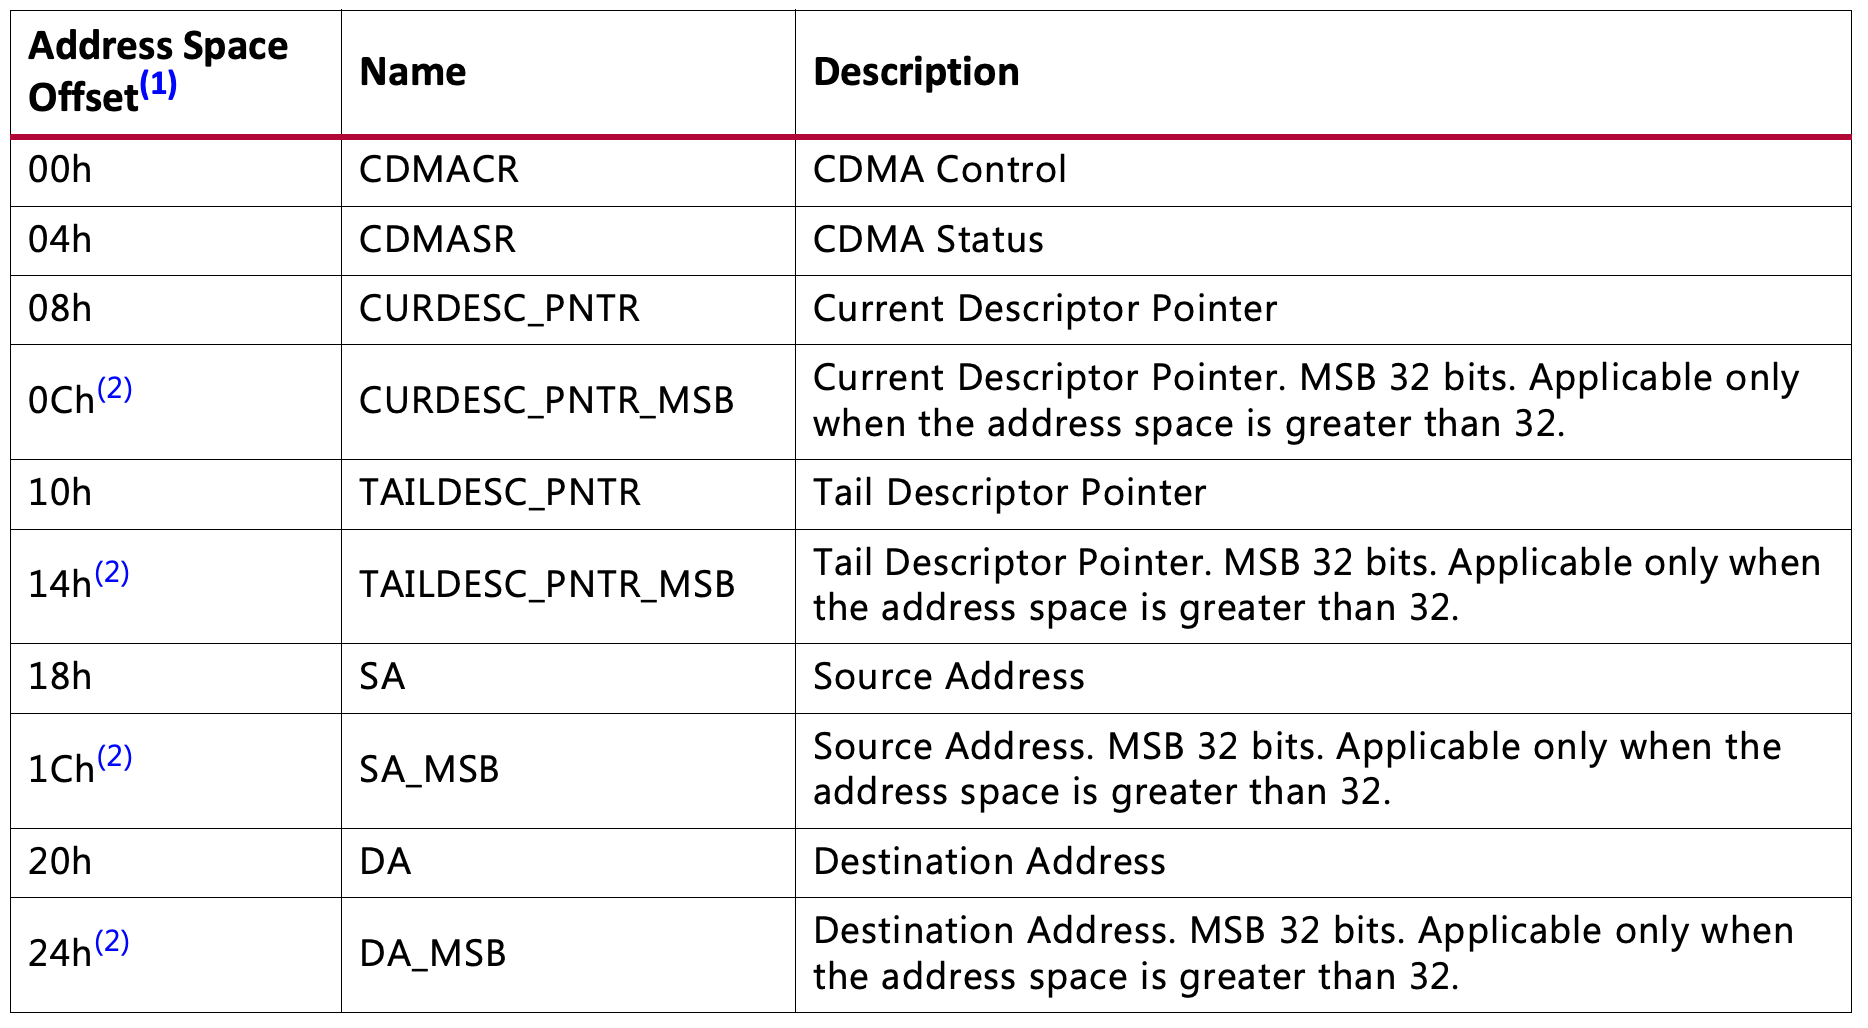
\includegraphics[width=0.8\textwidth]{fig/cmda_addrmap_1.png}
\caption{AXI CDMA Register Address map}
\label{fig4}
\end{figure}
\begin{figure}[htb!]
	\centering
	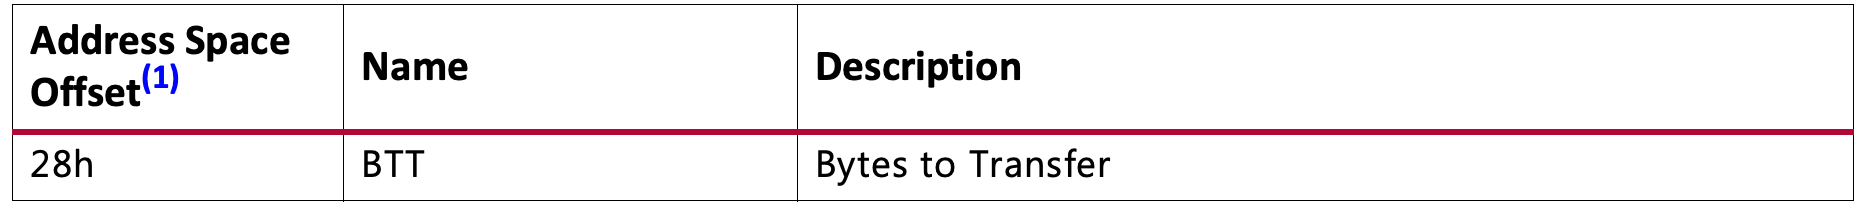
\includegraphics[width=0.8\textwidth]{fig/cdma_addrmap_2.png}
\caption{AXI CDMA Register Address map (cont.)}
\label{fig5}
\end{figure}

\newpage
\subsection*{\texttt{Memcopy \& Memory load, write}}
\begin{lstlisting}[style={c-style}]
struct timeval st[4];

// memory load
int foo;
foo = open("/dev/mem", O_RDWR);
float *ps_dram = mmap(NULL, (SIZE * (SIZE + 1))* sizeof(float), PROT_READ|PROT_WRITE, MAP_SHARED, foo, 0x10000000);

// MCPY: DRAM -> DRAM
gettimeofday (&st[0], NULL);
for (i = 0; i < SIZE * (SIZE + 1); i++)
    *(ps_dram + i) = flat[i];
gettimeofday (&st[1], NULL);
memcpy( ps_dram, flat, SIZE * (SIZE + 1) * sizeof(float) );
gettimeofday (&st[2], NULL);
\end{lstlisting}
\begin{itemize}
  \setlength\itemsep{-0.5em}
    \item  \texttt{mmap()} 함수를 통해, bitstream에서 미리 할당된 DRAM address(0x00000000 - 0x0000FFFF)를 메모리(ps\_dram)에 대응시킨다 (6번째 줄).
    \item for문을 통해 memory load를 수행한다 (10-11번째 줄).
    \item  \texttt{memcpy()} 함수를 통해 memory copy를 수행한다 (13번째 줄).
    \item  \texttt{gettimeofday()} 함수를 통해 수행시간을 측정한다 (9, 12, 14번째 줄).
\end{itemize}
memcpy와 for문을 이용한 memory load에서 memcpy가 더 좋은 수행시간을 가질 것이라 예상해 볼 수 있는데, 그 이유는 memcpy는 byte포인터가 아닌 word pointer를 이용하여 메모리 복사를 수행하고, SIMD (single instruction, multiple data)를 이용하여 assembly instruction을 수행하기 때문이다.

\section{Result}
\begin{figure}[htb!]
	\centering
	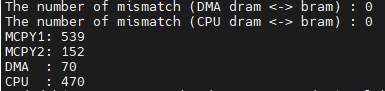
\includegraphics[width=0.7\textwidth]{fig/make2.png}
\caption{\texttt{for-loop}(\textit{MCPY1})/\texttt{memcpy}(\textit{MCPY2}) 비교, DMA/CPU memory load의 수행시간 (micro second) 비교: DMA를 사용하여 non-cacheable memory에서 BRAM으로 데이터를 전달하는 시간이 CPU의 내장함수 \texttt{memcpy} 보다 훨씬 (약 7배) 적은 시간 이 걸렸다.}
\label{fig6}
\end{figure}

주어진 main.c코드를 zedboard위에서 수행하였을 때, 수행속도는 DMA, memcpy (MCPY2), memory load (MCPY1)순으로 빠르게 나타난 것을 확인할 수 있었다. 실험을 진행하기 전 예상과 일치하였는데, 이는 DMA는 CPU를 거치지 않고 바로 memory에 접근하여 copy하여, c코드를 통해 구현한 memcpy, memory load보다 속도 측면에서 더 효율적이었다.
memcpy, memory load는 위에서 언급했듯, memcpy의 구현이 for loop를 통한 memory load보다 더 효율적이기 때문에 속도 측면에서 차이가 난 것이라 생각하였다.

\begin{figure}[htb!]
	\centering
	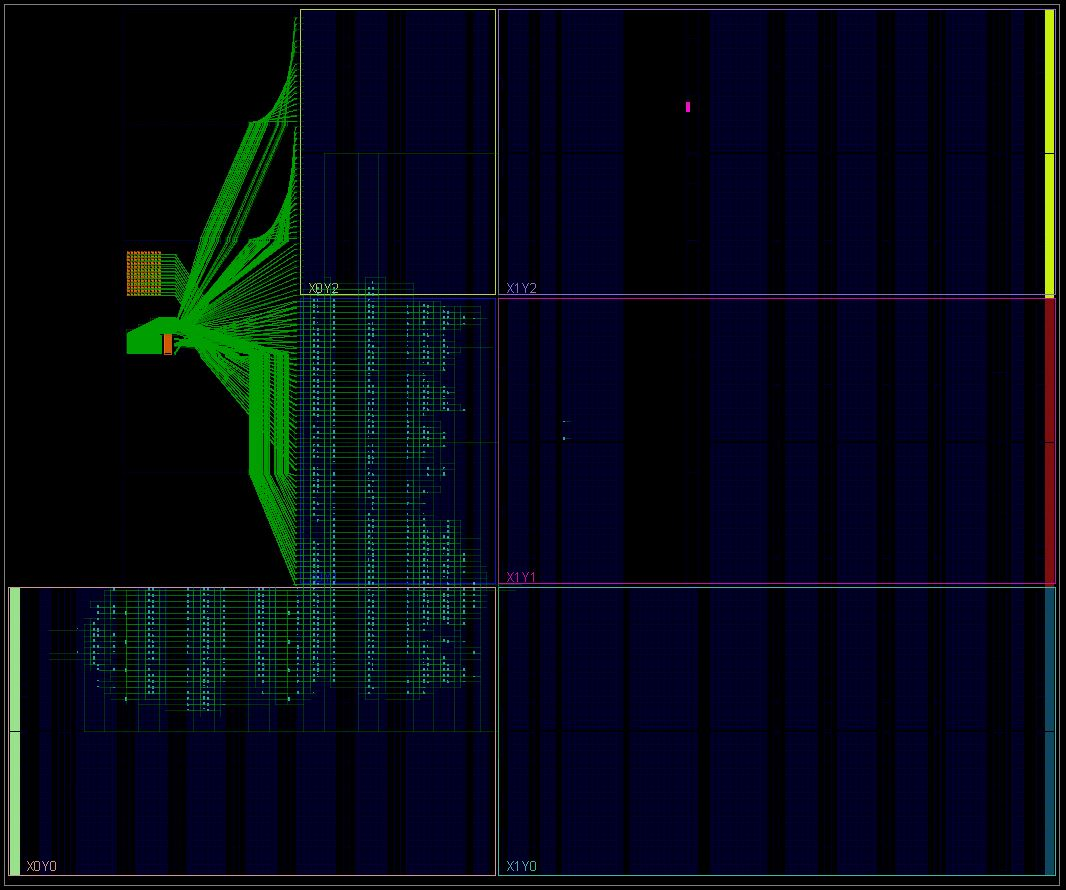
\includegraphics[width=0.7\textwidth]{fig/implementation.jpg}
\caption{Implementation, DMA 모듈을 함께 넣어 하드웨어 구현을 하였을 때의 모습이다.}
\label{fig7}
\end{figure}

\section{Conclusion}
이번 실습에서는 DMA를 사용해 수행시간을 일반적으로 사용하는 memory copy, load와 비교해 보았다.
우리는 최종적으로 CNN을 위한 Matrix-Matrix multiplication을 구현한다. 여기서, DMA를 사용한 memory load의 속도 개선은 결과적으로 training, inference time의 속도 개선을 의미한다. 따라서, 이번 실습을 토대로 최종 프로젝트의 optimization의 힌트를 얻을 수 있었다.

\bibliographystyle{plain}
\bibliography{other}

\end{document}
